\documentclass{beamer}
\usepackage{tikz}
\usepackage{wrapfig}
\usepackage{float}
\usepackage{multicol}
\usepackage{amsmath}
\usepackage[listings,theorems]{tcolorbox}

\setbeamercolor*{title}{use=structure,fg=white,bg=black}
\setbeamercolor*{author}{use=structure,fg=white}
\setbeamercolor*{date}{use=structure,fg=white}
\setbeamercolor{whitetext}{fg=white}

\title[Unravelling higher order chromatin organisation through statistical analysis] % (optional, only for long titles)
{ {\large Unravelling higher order chromatin organisation through statistical analysis } }
%\subtitle{ {\normalsize Second year report } }
\author[ \insertlogo{} ] 
{\vspace{15ex} \\
Ben Moore
\vspace{-4ex} }
% \institute[IGMM] 
% {
%   MRC HGU, IGMM
% }
\date{19$^{\mathrm{th}}$ November 2015}
\logo{
  \includegraphics[width=1.35cm]{figs/logo.png}
}
%\usetheme{Hannover}
\usetheme{Marburg}
\usecolortheme{dolphin}
%\usecolortheme{dove}

 %% End preamble

\begin{document}


{
\usebackgroundtemplate{\includegraphics[width=.85\paperwidth]{figs/hicbg_3.png}}
%\setbeamertemplate{sidebar left}{\logo{}}
\begin{frame}
%\hspace{-20em}
\titlepage
\end{frame}
}

% ----- Begin introduction

\section{Introduction}

\begin{frame}{Introduction}

Broad aim: investigate the relationship between structure and function of the genome

\vspace{2em}
Some specific questions:

\begin{enumerate}
\item How does higher order chromatin structure compare across human cell types?
\item Can we predict higher order chromatin structure from locus-level features?
\item How do the characteristics of boundaries demarcating higher order domains vary between cell types and domain classes?
\end{enumerate}

\end{frame}

\begin{frame}{What's known about genome structure}
\centering
\includegraphics[width=.8\textwidth]{../figs/genome_org.png}

\end{frame}

\begin{frame}{Hi-C: a genome-wide chromosome conformation assay }

\centering
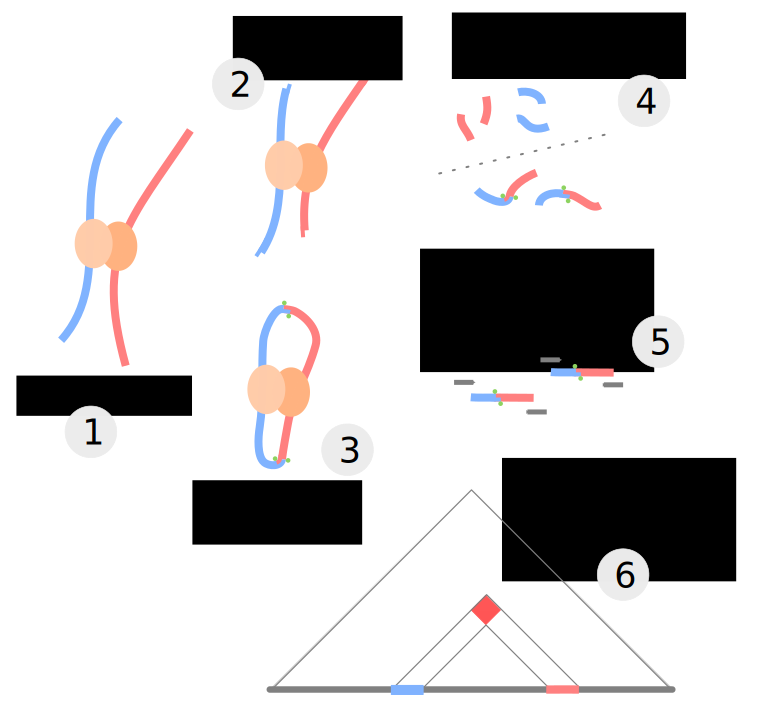
\includegraphics[width=.8\textwidth]{../figs/hic.png}

\end{frame}


\begin{frame}{Chromosome compartments from Hi-C data }

\centering
\includegraphics[width=.6\textwidth]{../figs/eigcalc.png}

\end{frame}

\begin{frame}{ Strategy }

{\small

\begin{itemize}
\item Integrate publicly available Hi-C data
\item Uniformly reprocess each dataset 
\item Call compartments, TADs from reprocessed data
\item Integrate cell-matched ENCODE epigenomic data
\end{itemize}

Then:
\begin{enumerate}
\item Compare/contrast cell types after reprocessing
\item Attempt predictive models of compartments and TADs from epigenomic features
\item Analyse boundary composition in terms of epigenomic features
\end{enumerate}

Related collaborative work:
\begin{enumerate}
\setcounter{enumi}{3}
\item Investigate concept of "metaTADs"
\item Analyse conformation changes at specific locus of interest 
\end{enumerate}
}

\end{frame}

% ----- End of introduction

% ----- Begin Reanalysis of Hi-C

\section{Reanalysis of Hi-C datasets}

\begin{frame}{Reanalysis of Hi-C datasets}
Very different sequencing depths between the input datasets: \\

\vspace{2em}

\centering
\includegraphics[width=.9\textwidth]{../figs/hicnorm.png}

\end{frame}

\begin{frame}{Reanalysis of Hi-C datasets}
Despite this, reprocessed Hi-C data is well-correlated: \\

\vspace{2em}

{\centering
\includegraphics[width=.9\textwidth]{../figs/blowout.png}
}
\vspace{2em}

Justifies going forward with between cell-line analysis

\end{frame}

\begin{frame}{Improved compartment calling algorithm}

\begin{columns}

\column{.4\textwidth}
\centering
\includegraphics[width=.85\textwidth]{../figs/hmm_flow.pdf}

\column{.6\textwidth}
\centering
\includegraphics[width=\textwidth]{../figs/hmm_calls.png}

\end{columns}

\end{frame}

\begin{frame}{Regions of variable compartment structure}

Regions of open, active compartment in one cell type but closed, repressive in the other two are enriched for cell type specific enhancer chromatin states: \\

\vspace{2em}

\centering
\includegraphics[width=.55\textwidth]{../figs/enhancerstates.pdf}

\end{frame}

\begin{frame}{Regions of variable compartment structure}

Some harbour genes with known cell type specific function

\vspace{1em}

\centering
\includegraphics[width=.55\textwidth]{../figs/examplervs.png}

\end{frame}



% ----- End Reanalysis of Hi-C

% ----- Begin Reanalysis of Hi-C


\begin{frame}{Main project}
Can model compartments, cross-apply between cell types: \\

\vspace{2em}

\centering
\includegraphics[width=.65\textwidth]{figs/f2.png}
\includegraphics[width=.35\textwidth]{figs/f3.png}

\end{frame}

\begin{frame}{Main project}
Lots of new boundary enrichments, quantitatively tested: \\

\vspace{1em}

\centering
\includegraphics[width=.75\textwidth]{figs/f6.png}

\end{frame}

\begin{frame}{Main project}
Currently in review: \\

\vspace{1em}

\centering

\includegraphics[width=.8\textwidth]{figs/inreview.png}
\end{frame}

\section{Collaborations}
\begin{frame}{Side project}
Collaborating with Adam Douglas (Bob Hill's group) in analysing his
3C-seq (4C) data. Their hypothesis: \\

\vspace{1em}

\centering

\includegraphics[width=.8\textwidth]{figs/tsa.png}
\end{frame}

\begin{frame}{Side project}
Initial results: \\

\vspace{1em}

\centering

\includegraphics[width=.9\textwidth]{figs/shh.pdf} \\
\end{frame}

\begin{frame}{Side project}
Zoomed: \\

\vspace{1em}

\centering

\includegraphics[width=.9\textwidth]{figs/zoomSHH.pdf} \\

Incoming: repeats, 5C / Capture-C (?), FAIRE-seq \dots
\end{frame}

\begin{frame}{Side project}
All looks good except\dots \\

\vspace{1em}

\centering

\includegraphics[width=.9\textwidth]{figs/csomeprop.pdf} \\

\end{frame}

\section{Next project}
\begin{frame}{Next project}
  So far haven't looked at any expression data, but CAGE available for
  each cell line. \\

\vspace{1em}

Initial idea:\\

\vspace{1em}

\begin{itemize}
\item Investigate TADs as ``regulons''---new paper reports $~20\%$
  domains act as ``discrete regulatory units'' with relatively
  homogenous epigenetic states.\footnote{ {\tiny Le Dily \emph{et al.} (2014) Distinct structural transitions of chromatin correlate with
  coordinated hormone-induced gene regulation. \emph{Genes and
    Development}, {\bf 28}:2151-62.} } 
\end{itemize}

\vspace{1em}

Can I find evidence for this with my data?
\end{frame}

\begin{frame}{Next project}
\centering
\includegraphics[width=.3\textwidth]{figs/venn.pdf} \\
\includegraphics[width=.5\textwidth]{figs/hgd.pdf}
\includegraphics[width=.5\textwidth]{figs/hist.pdf} 
\end{frame}

\begin{frame}{Next project}
\begin{itemize}
\item Higher resolution Hi-C now available, better for identifying domains
\item Improved methods of calling domains, where / why are some
  well-conserved between cell types?
\item Mouse data also available
\end{itemize}
\end{frame}


% \section{Year summary}
% \begin{frame}{Year summary}
% \vspace{-1em}
% \begin{enumerate}
% \item Completed main project on integrating uniformly-processed Hi-C and
%   ENCODE datasets (\emph{in review})
% \includegraphics[width=.8\textwidth]{figs/inreview.png}
% \item Presented related posters at ISMB (Boston) and Genome
%   Informatics (Cambridge); spoke at Edinburgh Bioinformatics
% \item Ongoing collaborations with wet-lab researchers (particularly
%   Adam Douglas in Bob Hill's group)
% \end{enumerate}
% \end{frame}

\section{Thesis plan}
\begin{frame}{Thesis plan p1}
\begin{enumerate}
\item Introduction
\item Methods
\item {\bf Modelling transcription and chromatin} Replicating and
  extending ENCODE project predicting txn output; adapt techniques to
  genome organisation
\item {\bf Model dissection} How the chromatin structure models
  cross-apply; regularised models; variable importance
\item {\bf Boundaries} Comparing TADs/compartments across boundaries;
  ``super bounds''; Giemsa bands
\item \dots
\end{enumerate}

\end{frame}

\begin{frame}{Thesis plan p2}
\begin{enumerate}
\setcounter{enumi}{5}
\item {\bf Investigating the function of self-interacting domains}
  Work from future project (very early stages); possibly two chapters
  from the next year
\item {\bf C-methods collaborations} Write-up Hill lab collaborations,
  possibly include other minor collabs
\item Discussion
\item End materials, code
\end{enumerate}

\end{frame}


\section{Acknowledgements}

{
\usebackgroundtemplate{\includegraphics[width=.85\paperwidth]{figs/hicbg_3.png}}
\begin{frame}{}
\begin{tcolorbox}[colback=blue!40!black,colframe=blue!40!black]
\begin{center}
{\usebeamercolor[fg]{whitetext}
{\small Thanks to supervisors:} \\ Colin Semple and
Stuart Aitken
}
\end{center}
\end{tcolorbox}

% \vspace{48pt}

% \begin{tcolorbox}[colback=blue!30,colframe=blue!40!black,title=Key references]
% \begin{tiny}
% \begin{itemize}
% \setlength{\itemindent}{-2em}
% \item[1.] Lieberman-Aiden, E. \emph{et al.} (2009) Comprehensive mapping
%   of long-range interactions reveals folding principles of the human
%   genome. \emph{Science}, {\bf 326}, p289-93.
% \item[2.] Kalhor, R. \emph{et al.} (2012) Genome architectures
%   revealed by tethered chromosome conformation capture and
%   population-based modeling. \emph{Nature biotechnology}, {\bf 30}, p90-98.
% \item[3.] Dixon, J.R. \emph{et al.} (2012) Topological domains in
%   mammalian genomes identified by analysis of chromatin
%   interactions. \emph{Nature}, {\bf 485}, p376-80.
% \item[4.] Yaffe, E. and Tanay, A. (2011) Probabilistic modeling of
%   Hi-C contact maps eliminates systematic biases to characterize
%   global chromosomal architecture. \emph{Nature genetics}, {\bf
%     43}:11, p1059-65.
% \end{itemize}
% \end{tiny}

% \end{tcolorbox}
\end{frame}
}

% \section{}
% \begin{frame}{Chromosome selection}
% \begin{figure}[H]
% \begin{center}
% \includegraphics[width=\textwidth]{figs/ChosenCsomes.png}
% \end{center} 
% \end{figure} 
% \end{frame}

% % \begin{frame}{Chromosomal compartments}
% % \begin{figure}[H]
% % \begin{center}
% % \includegraphics[width=\textwidth]{figs/compartCharact.pdf}
% % \end{center} 
% % \end{figure} 
% % \end{frame}

% \begin{frame}{Just more ``stuff'' binding in open comparments?}
% \begin{multicols}{3}
% \begin{figure}[H]
% \includegraphics[width=.33\textwidth]{figs/gshuff.pdf}
% \end{figure} 
% \columnbreak
% \begin{figure}[H]
% \includegraphics[width=.33\textwidth]{figs/hshuff.pdf}
% \end{figure} 
% \columnbreak
% \begin{figure}[H]
% \includegraphics[width=.33\textwidth]{figs/kshuff.pdf}
% \end{figure} 
% \end{multicols}

% Here the eigenvector values are shuffled per compartment type.
% \end{frame}

\end{document}